\documentclass{report}

\input{preamble}
\input{macros}
\input{letterfonts}

\title{\Huge{Some Class}\\Random Examples}
\author{\huge{Your Name}}
\date{}

\begin{document}

\maketitle
\newpage% or \cleardoublepage
% \pdfbookmark[<level>]{<title>}{<dest>}
\pdfbookmark[section]{\contentsname}{toc}
\tableofcontents
\pagebreak

\chapter{}
\section{Random Examples}
\dfn{Limit of Sequence in $\bs{\bbR}$}{Let $\{s_n\}$ be a sequence in $\bbR$. We say $$\lim_{n\to\infty}s_n=s$$ where $s\in\bbR$ if $\forall$ real numbers $\eps>0$ $\exists$ natural number $N$ such that for $n>N$ $$s-\eps<s_n<s+\eps\text{ i.e. }|s-s_n|<\eps$$}
\qs{}{Is the set ${x-}$axis${\setminus\{\text{Origin}\}}$ a closed set}
\sol We have to take its complement and check whether that set is a open set i.e. if it is a union of open balls
\nt{We will do topology in Normed Linear Space  (Mainly $\bbR^n$ and occasionally $\bbC^n$)using the language of Metric Space}
\clm{Topology}{}{Topology is cool}
\ex{Open Set and Close Set}{
	\begin{tabular}{rl}
		Open Set:   & $\bullet$ $\phi$                                              \\
		            & $\bullet$ $\bigcup\limits_{x\in X}B_r(x)$ (Any $r>0$ will do) \\[3mm]
		            & $\bullet$ $B_r(x)$ is open                                    \\
		Closed Set: & $\bullet$ $X,\ \phi$                                          \\
		            & $\bullet$ $\overline{B_r(x)}$                                 \\
		            & $x-$axis $\cup$ $y-$axis
	\end{tabular}}
\thm{}{If $x\in$ open set $V$ then $\exists$ $\delta>0$ such that $B_{\delta}(x)\subset V$}
\begin{myproof}By openness of $V$, $x\in B_r(u)\subset V$
	\begin{center}
		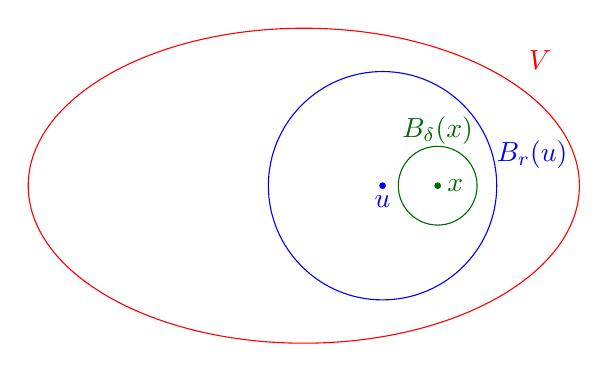
\begin{tikzpicture}
			\draw[red] (0,0) circle [x radius=3.5cm, y radius=2cm] ;
			\draw (3,1.6) node[red]{$V$};
			\draw [blue] (1,0) circle (1.45cm) ;
			\filldraw[blue] (1,0) circle (1pt) node[anchor=north]{$u$};
			\draw (2.9,0.4) node[blue]{$B_r(u)$};
			\draw [green!40!black] (1.7,0) circle (0.5cm) node [yshift=0.7cm]{$B_{\delta}(x)$} ;
			\filldraw[green!40!black] (1.7,0) circle (1pt) node[anchor=west]{$x$};
		\end{tikzpicture}
	\end{center}

	Given $x\in B_r(u)\subset V$, we want $\delta>0$ such that $x\in B_{\delta} (x)\subset B_r(u)\subset V$. Let $d=d(u,x)$. Choose $\delta $ such that $d+\delta<r$ (e.g. $\delta<\frac{r-d}{2}$)

	If $y\in B_{\delta}(x)$ we will be done by showing that $d(u,y)<r$ but $$d(u,y)\leq d(u,x)+d(x,y)<d+\delta<r$$
\end{myproof}

\cor{}{By the result of the proof, we can then show...}
\mlenma{}{Suppose $\vec{v_1}, \dots, \vec{v_n} \in \RR[n]$ is subspace of $\RR^n$.}
\mprop{}{$1 + 1 = 2$.}

\section{Random}
\dfn{Normed Linear Space and Norm $\boldsymbol{\|\cdot\|}$}{Let $V$ be a vector space over $\bbR$ (or $\bbC$). A norm on $V$ is function $\|\cdot\|\ V\to \bbR_{\geq 0}$ satisfying \begin{enumerate}[label=\bfseries\tiny\protect\circled{\small\arabic*}]
		\item \label{n:1}$\|x\|=0 \iff x=0$ $\forall$ $x\in V$
		\item \label{n:2}	$\|\lambda x\|=|\lambda|\|x\|$ $\forall$ $\lambda\in\bbR$(or $\bbC$), $x\in V$
		\item \label{n:3} $\|x+y\| \leq \|x\|+\|y\|$ $\forall$ $x,y\in V$ (Triangle Inequality/Subadditivity)
	\end{enumerate}And $V$ is called a normed linear space.

	$\bullet $ Same definition works with $V$ a vector space over $\bbC$ (again $\|\cdot\|\to\bbR_{\geq 0}$) where \ref{n:2} becomes $\|\lambda x\|=|\lambda|\|x\|$ $\forall$ $\lambda\in\bbC$, $x\in V$, where for $\lambda=a+ib$, $|\lambda|=\sqrt{a^2+b^2}$ }


\ex{$\bs{p-}$Norm}{\label{pnorm}$V={\bbR}^m$, $p\in\bbR_{\geq 0}$. Define for $x=(x_1,x_2,\cdots,x_m)\in\bbR^m$ $$\|x\|_p=\Big(|x_1|^p+|x_2|^p+\cdots+|x_m|^p\Big)^{\frac1p}$$(In school $p=2$)}
\textbf{Special Case $\bs{p=1}$}: $\|x\|_1=|x_1|+|x_2|+\cdots+|x_m|$ is clearly a norm by usual triangle inequality. \par
\textbf{Special Case $\bs{p\to\infty\ (\bbR^m$ with $\|\cdot\|_{\infty})}$}: $\|x\|_{\infty}=\max\{|x_1|,|x_2|,\cdots,|x_m|\}$\\
For $m=1$ these $p-$norms are nothing but $|x|$.
Now exercise
\qs{}{\label{exs1}Prove that triangle inequality is true if $p\geq 1$ for $p-$norms. (What goes wrong for $p<1$ ?)}
\sol{\textbf{For Property \ref{n:3} for norm-2}	\subsubsection*{\textbf{When field is $\bbR:$}} We have to show\begin{align*}
		         & \sum_i(x_i+y_i)^2\leq \left(\sqrt{\sum_ix_i^2} +\sqrt{\sum_iy_i^2}\right)^2                                       \\
		\implies & \sum_i (x_i^2+2x_iy_i+y_i^2)\leq \sum_ix_i^2+2\sqrt{\left[\sum_ix_i^2\right]\left[\sum_iy_i^2\right]}+\sum_iy_i^2 \\
		\implies & \left[\sum_ix_iy_i\right]^2\leq \left[\sum_ix_i^2\right]\left[\sum_iy_i^2\right]
	\end{align*}So in other words prove $\langle x,y\rangle^2 \leq \langle x,x\rangle\langle y,y\rangle$ where
	$$\langle x,y\rangle =\sum\limits_i x_iy_i$$

	\begin{note}
		\begin{itemize}
			\item $\|x\|^2=\langle x,x\rangle$
			\item $\langle x,y\rangle=\langle y,x\rangle$
			\item $\langle \cdot,\cdot\rangle$ is $\bbR-$linear in each slot i.e. \begin{align*}
				      \langle rx+x',y\rangle=r\langle x,y\rangle+\langle x',y\rangle	\text{ and similarly for second slot}
			      \end{align*}Here in $\langle x,y\rangle$ $x$ is in first slot and $y$ is in second slot.
		\end{itemize}
	\end{note}Now the statement is just the Cauchy-Schwartz Inequality. For proof $$\langle x,y\rangle^2\leq \langle x,x\rangle\langle y,y\rangle $$ expand everything of $\langle x-\lambda y,x-\lambda y\rangle$ which is going to give a quadratic equation in variable $\lambda $ \begin{align*}
		\langle x-\lambda y,x-\lambda y\rangle & =\langle x,x-\lambda y\rangle-\lambda\langle y,x-\lambda y\rangle                                       \\
		                                       & =\langle x ,x\rangle -\lambda\langle x,y\rangle -\lambda\langle y,x\rangle +\lambda^2\langle y,y\rangle \\
		                                       & =\langle x,x\rangle -2\lambda\langle x,y\rangle+\lambda^2\langle y,y\rangle
	\end{align*}Now unless $x=\lambda y$ we have $\langle x-\lambda y,x-\lambda y\rangle>0$ Hence the quadratic equation has no root therefore the discriminant is greater than zero.

	\subsubsection*{\textbf{When field is $\bbC:$}}Modify the definition by $$\langle x,y\rangle=\sum_i\overline{x_i}y_i$$Then we still have $\langle x,x\rangle\geq 0$}

\section{Algorithms}
\begin{algorithm}[H]
\KwIn{This is some input}
\KwOut{This is some output}
\SetAlgoLined
\SetNoFillComment
\tcc{This is a comment}
\vspace{3mm}
some code here\;
$x \leftarrow 0$\;
$y \leftarrow 0$\;
\uIf{$ x > 5$} {
    x is greater than 5 \tcp*{This is also a comment}
}
\Else {
    x is less than or equal to 5\;
}
\ForEach{y in 0..5} {
    $y \leftarrow y + 1$\;
}
\For{$y$ in $0..5$} {
    $y \leftarrow y - 1$\;
}
\While{$x > 5$} {
    $x \leftarrow x - 1$\;
}
\Return Return something here\;
\caption{what}
\end{algorithm}

\end{document}
